

\section{Stage 2: Orchestrator} \label{sec:work_stage2_orchestrator}




Having all the benchmarks generated, it is possible to move to the next stage. Gathering the energy profiles for each of the generated benchmarks. 
Energy profiles~\cite{10.1145/2884781.2884869,8816747} are an established way to organize energy consumption data. They will be the main data source of the machine learning models to obtain accurate results. To reduce the complexity of this task, a process was implemented, illustrated in Figure~\ref{fig:orchestrators_workflow}. This process automates the task while taking into account what was mentioned in Section~\ref{sec:background_benchmarking}.

As described in the Section~\ref{sec:background_energy} there are several tools capable of performing dynamic energy measurements.

PowerJoular has good features that caught our attention, for example being a command line tool that could be easily integrated in almost every programming language, it stores the energy used in a CSV file, capable of only reading energy of running processes and so on, as explained before in Section~\ref{sec:background_energy}.

Since PowerJoular is a command line tool, it is launched as a process, and then it can be killed whenever needed because it is a process as well. This allows to measure not only programs/processes energies but have a more precise measurement, as it is possible to call PowerJoular to measure a specific computation and then kill it when the computation is finished.

With all of this in mind a process was built. The process uses an orchestrator that is responsible for invoking the target benchmark and the measurement tool (PowerJoular) to accurately measure the energy consumption of the benchmark or the specific computation being analyzed within it.


One challenge in measuring energy consumption is that computation often completes too quickly to capture accurately. It is hard to measure a single operation of, for example, a \texttt{List.\allowbreak add(Object)} with most tools, as it simply to fast for the tool to capture, and if the tool was able to capture it, the energy measured could have too much noise to be considered. Our solution was to loop through the method until the tool is capable of getting its energy and then dividing the total energy by the number of times it looped. 
This solution, although effective, introduces potential errors that need to be addressed.

By approaching the measurements with the loop technique, first we need to create the variables needed for the method target to analysis, like shown in the Listing~\ref{lst:var_placeholders} \begin{comment}\wo{dê exemplos}\end{comment}. However, because, the methods are treated like a black box, it is not possible to know what the methods are going to do with the parameters or with its variables.  For example, the method \texttt{List.size()} has no parameteres, and return the size of the list. In this case the functioning of the method is known, and it is noticeable that the attributes of the object will not change, as the method simply reads and returns a value.

However, this raises problems with other methods, such as \texttt{List.add(Object)}. This method will insert values in the list, increasing its size. This increase in size can lead to different behavior of the method as the internal object changes in each iteration. In this case, inserting into a smaller list can produce different measurements of inserting into a larger list.

Now, suppose we have a method called \texttt{sort} that takes a randomly ordered list and sorts it. This introduces a problem when measuring its energy consumption. On the first run, the method will sort the unsorted list, which may take significant time depending on the randomness of the data and the sorting algorithm used. However, on subsequent runs with the same list, the input is already sorted, meaning the sort method will likely complete much faster or with minimal effort. This difference can result in misleading or inconsistent measurements.

To prevent this side effect from happening we designed a solution that consists of creating an array that holds the parameters, that can be seen in the Figure~\ref{fig:array}. The necessary parameters to execute the method are created and stored into the array. They are exactly copies with different refereces. Now, if one of the elements is changed during its execution on the method, it will not affect the other's execution. Since this approach increases memory usage due to multiple copies, we empirically selected array sizes (75,000, 100,000, and 150,000) to balance between avoiding out-of-memory errors and ensuring the computation runs long enough for PowerJoular to record energy measurements. PowerJoular by default needs to run for 1 second to create the CSV file that has the energy used for the target process, so these sizes aim so that looping the array takes at least a second. In some cases, the CSV file may not be generated because the loop executes too quickly. In such instances, the energy reading will be assumed to be 0 J, as the execution was too fast to record a value.


\begin{figure}[htbp]
  \centering
  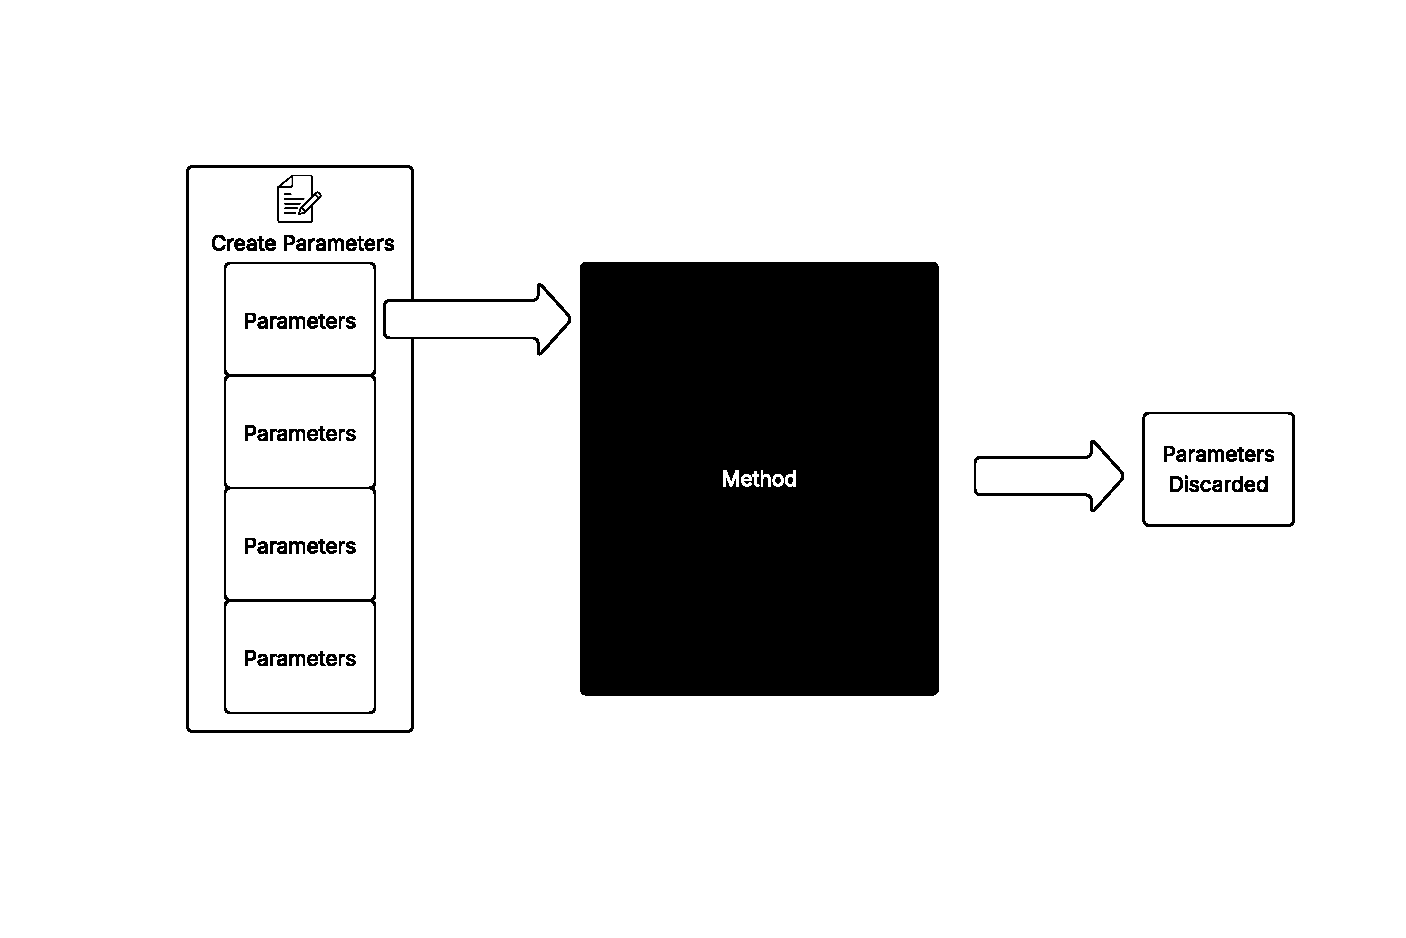
\includegraphics[width = 1 \textwidth]{figures/array.pdf}
  \caption{Array example}
  \label{fig:array}
\end{figure}

To be able to collect some faster executions, the original PowerJoular was modified to allow customizable measurement durations, enabling readings at intervals shorter than the default 1 second, such as 100ms, which provides greater flexibility and finer granularity in energy profiling.

The computation method shown in Listing~\ref{lst:Computation_method} illustrates how each profiling method operates independently of the specific method being evaluated. It attempts to execute the target function repeatedly for approximately one second. In this particular case, the target function performs the operation \texttt{var.add(arg0);} and returns the number of iterations completed, which is then used for further calculations.

\begin{listing}[htbp]%[H]
\noindent\rule{\linewidth}{0.4pt}
\begin{minted}[linenos, fontsize=\small, frame=none, bgcolor=white,breaklines=true,breakanywhere=true]{java}
private static int computation(BenchmarkArgs[] args, int iter) {
        int i = 0;
        while (!TemplatesAux.stop && i < iter) {
              arrayList_add_java_lang_Object_(args[i].var0, args[i].var1);
               i++;
        }
        return iter;
    }
\end{minted}
\noindent\rule{\linewidth}{0.4pt}
\caption{Computation method}            
\label{lst:Computation_method}
\end{listing}


With the process structure now defined, we can proceed to explain how it functions.

The workflow of this step can be described as follows:


\begin{figure}[htbp]
  \centering
  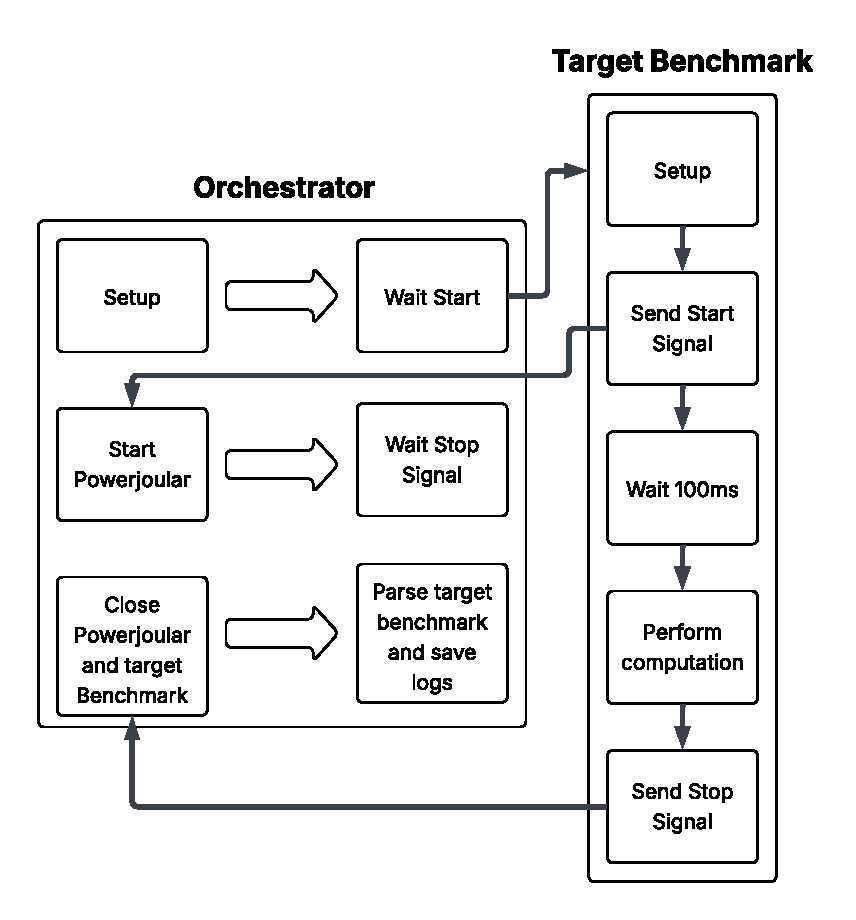
\includegraphics[scale = 0.7]{figures/orchestrators_process.pdf}
  \caption{Orchestrator Workflow}
  \label{fig:orchestrators_workflow}
\end{figure}

\begin{itemize}
  \item The orchestrator launches a command to start the target Java benchmark and waits a signal.
  \item The Java benchmark starts and setup the necessary elements to run (creating all the variables, reading/writing files, populating the array, etc.) and then before starting the computation it wants to measure, it sends a start signal to the orchestrator to start monitoring, and waits for 100 milliseconds.
  \item The orchestrator receives the start signal and reads the PID, which is stored in a file during the target benchmark setup. Finally, it starts PowerJoular using that PID. Then it waits for the stop signal.
  \item The Java benchmark will run until it finishes the computation. The computation runs for a maximum of one second. Then the number of iterations are stored in a file and the stop signal is sent back to the orchestrator.
  \item The orchestrator on receiving the stop signal, first stops PowerJoular and then stops the target benchmark, if needed. Then it parses the target benchmark to extract its features, combines them with the energy information stored in the files created by PowerJoular, stores it in a CSV file.
\end{itemize}

All these steps are performed for each generated benchmark. At the end of the process, a log file is created containing key information, including all the benchmarks used, the PowerJoular files generated, temporary files, error logs, and features.
